\documentclass{beamer}
\setbeamertemplate{headline}[frame number]
\setbeamertemplate{section in toc}[sections numbered]
\setbeamertemplate{subsection in toc}[subsections numbered] 
\usetheme[left, hideallsubsections]{Goettingen} 
\usepackage[utf8]{inputenc}
\usepackage{amsmath}
 
 
\title{Group 6\\
	Pond Environmental Measurement\\
	SSNS - Smart Sensor Network Systems}
\author{Alexander K.,
	Sabrina B.,
	Rozana A.,
	Alexander V.D.}
 
\institute[FHF] {Fachhochschule Frankfurt am Main - University of Applied Sciences}

\date 
{\today}

\begin{document}

\maketitle
\begin{frame}
\frametitle{Table of Contents}
\tableofcontents
\end{frame}

%%%%%%%%%%%%%%%%%%%%%%%%%%%%%%% Project Describtion %%%%%%%%%%%%%%%%%%%%%%%%%%%%%%%%%%
\section{Project Describtion} 
\subsection{Idea}
\frame
{
	\frametitle{Project}
	\begin{figure}[h!]
  		\centering
    	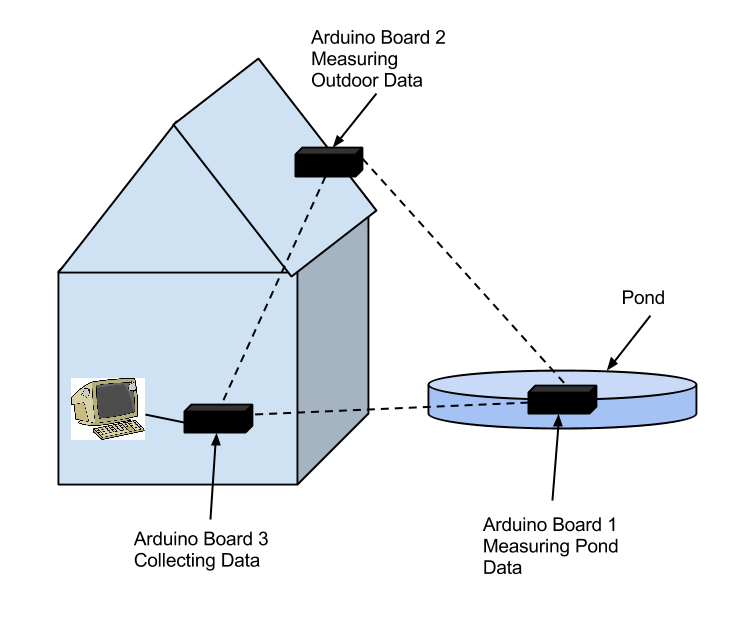
\includegraphics[width=0.85\textwidth]{../Images/ssns_project.png}
		\caption{Model}
	\end{figure}
}

%\frame
%{
%	\frametitle{Project}
%	\begin{itemize}
%	\item based on Wireless Smart Sensor Network
%	\item measure ponds water temperature
%	\item measure weather condition (Temperature and Light)
%	\item realizied with Arduino Boards and ZigBee Module
%	\end{itemize}
%}
%
%\frame
%{
%	\frametitle{Project}
%	The System consists of following Components :\\
%	\begin{itemize}
%	\item underwater Temperature measuring Sensor Node
%	\item over water weather measuring Node (Temperature, Light)
%	\item indoor Node collecting and storing the measured Data
%	\item A PC running a visualizing Application
%	\end{itemize}	
%}

\subsection{Requirements}
\frame
{
	\frametitle{System Requirements}
	\begin{itemize}
	\item reliable 24/7 data Aquisition
	\item Data being storaged on the collecting Node
	\item Graphical visualization on the PC
	\end{itemize}
}

%%%%%%%%%%%%%%%%%%%%%%%%%%%%%%% Estimation %%%%%%%%%%%%%%%%%%%%%%%%%%%%%%%%%%%%%%%%%%%%%
\section{Function Point Analysis}
\frame
{
	\frametitle{Function Points}
	\begin{enumerate}
	\item Defining the Unadjusted Function Point Count
	\item Determining the Value Adjustment Factor
	\item Determining Function Points
	\end{enumerate}
}

\subsection{Defining the Unadjusted Function Point Count}
\frame
{
	\frametitle{Defining the Unadjusted Function Point Count}
	\begin{figure}[h!]
  		\centering
    	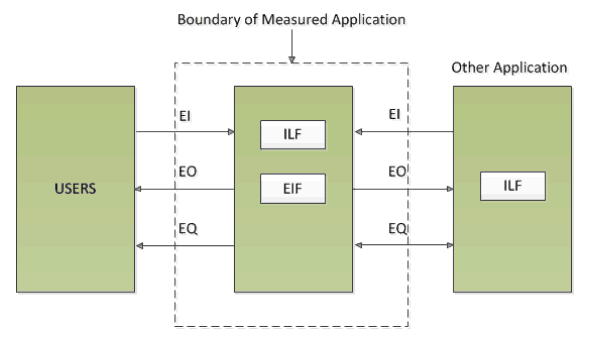
\includegraphics[width=0.85\textwidth]{../Images/FP_model.png}
		\caption{Boundary of MA}
	\end{figure}
}

\frame
{
	\frametitle{Unadjusted Function Point Count and Multipliers}
	\begin{figure}[h!]
  		\centering
    	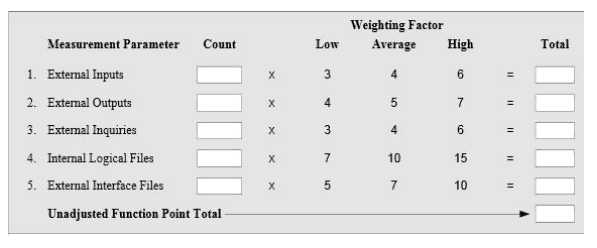
\includegraphics[width=\textwidth]{../Images/FP.png}
	\end{figure}
}

\subsection{Determinig the Value Adjustment Factor}
\frame
{
	\frametitle{Determinig the Value Adjustment Factor}	
	\begin{figure}[h!]
  		\centering
    	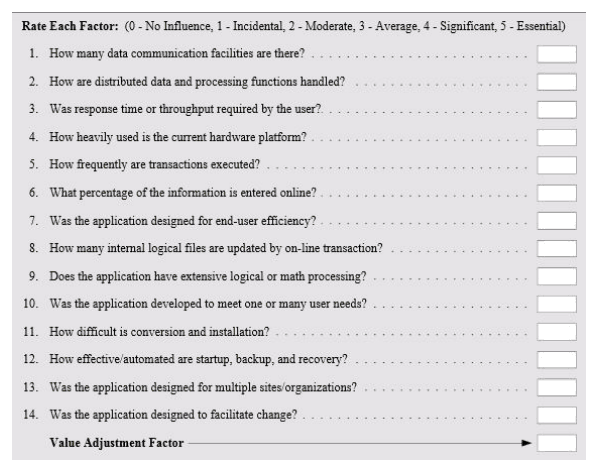
\includegraphics[width=0.85\textwidth]{../Images/FP_2.png}
		\caption{Total Degree of Influence}
	\end{figure}
}

\subsection{Determining Function Points}
\frame
{
	\frametitle{Determining Function Points}
	\begin{tabular}{|l|l|l|}
	\hline
	Project & Function Points 	& Man-Months 	\\ \hline
	ASD 	& 11 				& 1				\\ \hline
	KWO 	& 24 				& 2				\\ \hline
	RMD 	& 53 				& 5				\\ \hline
	WBO 	& 72 				& 6				\\ \hline
	\end{tabular}
}

\frame
{
	\frametitle{Determining Function Points}
	\begin{tabular}{|l|l|l|}
	\hline
	Project & Function Points 	& Man-Months 	\\ \hline
	ASD 	& 11 				& 1				\\ \hline
	Arduino	& 22				& 1.2			\\ \hline
	KWO 	& 24 				& 2				\\ \hline
	RMD 	& 53 				& 5				\\ \hline
	WBO 	& 72 				& 6				\\ \hline
	\end{tabular}
}

%%%%%%%%%%%%%%%%%%%%%%%%%%%%%%% System Architecture %%%%%%%%%%%%%%%%%%%%%%%%%%%%%%%%%%
\section{System Architecture}
\subsection{The Sensor}
\frame
{
	\frametitle{The Sensors}
	We are using two Sensors:	
	\begin{itemize}
	\item Temperature Sensor TMP36
	\item Light Dependant Resistor GL5528	
	\end{itemize}
}

\frame
{
	\frametitle{Temperature Sensor}
	\begin{figure}[h!]
  		\centering
    	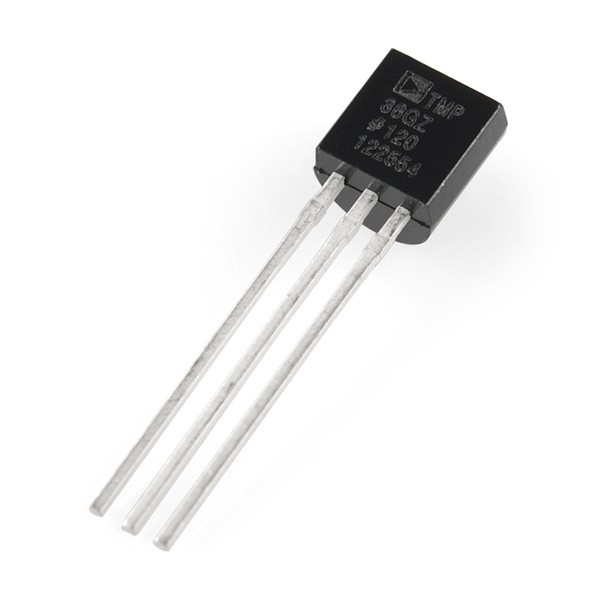
\includegraphics[width=0.5\textwidth]{../Images/Temp.jpg}
		\caption{TMP36}
	\end{figure}
}

\frame
{
	\frametitle{Temperature Sensor}
	Following Specification:
	\begin{itemize}
	\item outputs voltage depending on the temperature
	\item relation is linear
	\item Temperature Range: $-40^{\circ}$C to $125^{\circ}$C
	\item scalefactor of 10mV/$^{\circ}$C
	\item Accuracy of $\pm1^{\circ}$C at 25$^{\circ}$ and $\pm2\%$ in the range of $-40^{\circ}$C to 125$^{\circ}$C
	\end{itemize}
}

\frame
{
	\frametitle{Temperature Sensor}
	To calculate the Temperature in $^{\circ}$Celsius we use the formula:\\
	\begin{equation*}
	Temp = \frac{Voltage - 500}{10} 
	\end{equation*}
}

\frame
{
	\frametitle{Light Dependant Resistor}
		\begin{figure}[h!]
  		\centering
    	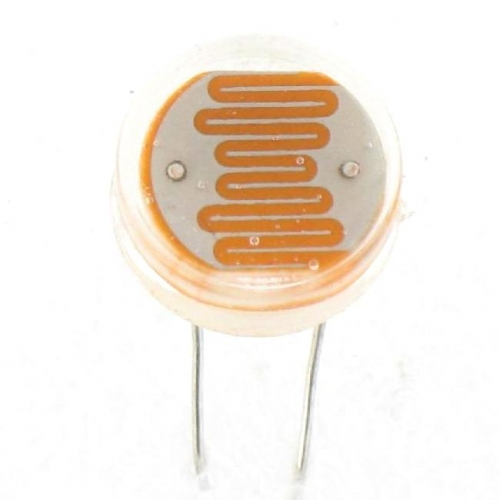
\includegraphics[width=0.5\textwidth]{../Images/Light.jpg}
		\caption{GL5528}
	\end{figure}
}

\frame
{
	\frametitle{Light Dependant Resistor}
	Following Specification:
	\begin{itemize}
	\item not precise enough to measure the light level
	\item only measure darkness from lightness
	\item Reliable perfomance
	\item linear relation
	\end{itemize}
}

\frame
{
	\frametitle{Light Dependant Resistor}
	To get the light value in Lux you have to do following steps:
	\begin{enumerate}
	\item Get Voltage of Resistor
	\item Get Resistor Value with formula:
	\begin{equation*}
		\frac{5.0 - Light Voltage}{lightv} * 10000
	\end{equation*}
	\item Get Lux with formula:
	\begin{equation*}
		10*\frac{14000}{Light Resistor}^\frac{1}{0.7}
	\end{equation*}
	\end{enumerate}
}

\frame
{
	\frametitle{Error Calculation}
	\begin{itemize}
	\item calculate quantisation error
	\item Temperature: $\pm$1 Degree
	\item Light: too high $\rightarrow$ only measure dark or bright of light
	\end{itemize}
}

\subsection{ZigBee Network}
\frame
{
	\frametitle{ZigBee Network}
	
	\begin{itemize}
	
	\item The Nodes in our WSN communicate in a ZigBee Network
	\item ZigBee Networks need a coordinator. The Collector will be the coordinator.
	\item The measuring Nodes will function either as End-Nodes or Routers
	\begin{itemize}
		\item{For the programming of the Nodes, this is irrelevant}
	\end{itemize}
	
	\end{itemize}
}

\frame
{
	\begin{itemize}
	
	\item As Radio Modules we are using XBee Modules from Digi
	\item They are attached to the Arduino's using Wireless Shields.
	\item To Adress the XBee Modules in the Software, we use the xbee-arduino Library
	\item The ZigBee adress of the coordinator will be hardcoded into the measuring Nodes Software
	\item The ZigBee Adress of the Measuring Nodes will be hard coded into the Coordinators Software
	\end{itemize}
}

\frame
{
	\frametitle{Communication}

	\begin{itemize}
	\item The coordinator will request Measurements from the Measuring Nodes
	\item The Message looks like this:
	\end{itemize}
	
	\begin{table}
    \begin{tabular}{|l|l|l|}
    \hline
    Byte(s) & content  & meaning                            \\ \hline
    1       & 'R'=0x52 & identifier for Measurement Request \\ \hline
    \end{tabular}
	\end{table}
}


\frame
{

	\begin{itemize}
	
	\item On Request, the Pond Measuring Node will Respond by this Message:
	
	\end{itemize}
	
	\begin{table}
    \begin{tabular}{|p{3cm}|p{3cm}|p{3cm}|}
    \hline
    Byte(s) & content  & meaning                                      \\ \hline
    1       & 'W'=0x57 & identifier for Measurement response          \\ \hline
    2-5     & float    & float for temperature measurement in Celsius \\ \hline
    6-9     & float    & float for light intensity in Lux             \\ \hline
    \end{tabular}
	\end{table}
}

\frame
{
	\begin{itemize}
	\item The Weather Measuring Node Responds with this Message:
	\end{itemize}
	
	\begin{table}[h]
    \begin{tabular}{|p{3cm}|p{3cm}|p{3cm}|}
    \hline
    Byte(s) & content  		& meaning                            \\ \hline
    1       & ''P'= 0x50 	& identifier for Pond measuremnt response \\ \hline
    2-5		& float			& float for temperature measurement in Celsius \\ \hline
    \end{tabular}
	\end{table}
}

\subsection{The Collecting Node}
\frame
{
	\frametitle{The Collecting Node}
	
	\begin{itemize}
	
	\item The collecting Node will take the following Responsibilities
	
	\begin{itemize}
	
	\item ZigBee coordinator Role
	\item Know Time by using NTP
	\item Request and Receive Measures and store them
	\item act as TCP Server, providing stored Data to clients
	
	\end{itemize}
	
	\item The collector consists of an Arduino Ethernet, with the same 
	Wireless Shield and XBee Module like the other Nodes, and an attached SD Card
	
	\end{itemize}

}

\subsection{The Measuring Nodes}

\frame
{
	\frametitle{The Measuring Nodes}
	\begin{itemize}
	\item Measurement Kit $\rightarrow$ Arduino Uno + Wireless Shield + XBee Module + 	Sensor Module	
	\item Sensor Module is different for Pond and Weather Measurement Station
	\item act as an ZigBee EndNode
	\item check if Coordinator has sent request
	\item if true send response to Coordinator	
	\end{itemize}
}

\frame
{
	\frametitle{The Measuring Nodes}
	\begin{figure}[h!]
  		\centering
    	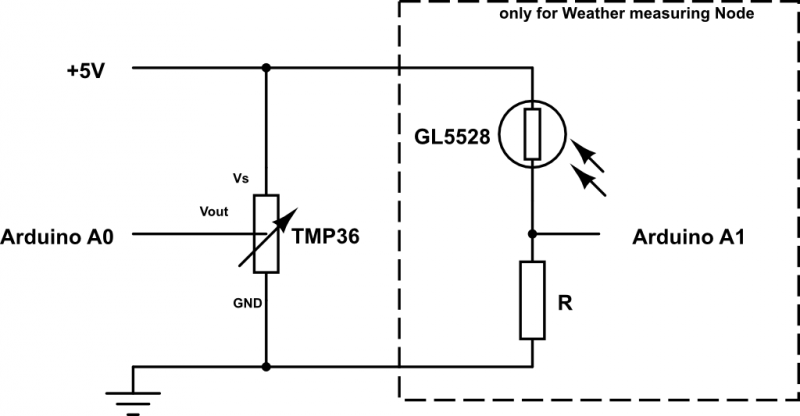
\includegraphics[width=\textwidth]{../Images/Circuit.png}
		\caption{Measuring Node Circuit}
	\end{figure}
}


\frame
{
	\frametitle{Behaviour}

	\begin{itemize}
	
	\item on startup, and every 24 hours, the collector will synchronize its time via NTP
	\item every full and half hour, the collector will request a Measurement from the Measuring Nodes
	\item The measuring Nodes have 30 Seconds to respond, otherwise their measurement is ignored
	\item After 30 seconds, or when the Measuring Nodes all answered, the measurements get stored.
	
	\end{itemize}

}


\frame
{
	\frametitle{Data Storage}

	\begin{itemize}
	
	\item The collector stores the Data in a File on its SD Card
	
	\item The File is a CSV-File (Coma separated Values) with the following Format:
	
	\item \textbf{hh,mm,ss,dd,mm,yyyy,pppp,aaaa,llll}
	
	\item Each Line represents a complete measurement of the system
	\item New measurements add lines to the File
	
	\end{itemize}
}

\frame
{
	\begin{itemize}
	\item missing values will be left out (but comas stay)
	
	\item Example:
	
	\item \textbf{00,30,15,13,05,2013,11.5,9.7,}
	
	\item Means: At 00:30:15 on the 13th of May 2013, the Pond Temperature was 11.5C, the air temperature was 9.7 C, and the light level was unknown
	\end{itemize}
}

\subsection{Application}
\frame
{
	\frametitle{Application}
	
	\begin{itemize}
	
	\item The application is used to access the collected data from the WSN
	
	\item The Data is displayed in a Table
	
	\item The Data can then be exportet as the same CSV File as stored on the collector
	
	
	\item The exportet File can then be used in other applications like GNUPlot or SciLab.
	
	\end{itemize}

}




%%%%%%%%%%%%%%%%%%%%%%%%%%%%%%% End %%%%%%%%%%%%%%%%%%%%%%%%%%%%%%%%%%%%%%%%%%%%%%%%%%%%
\frame
{
	\begin{center}
	Thank you for your attention!
	\end{center}
}

\end{document}
       
 